\section{Cấu trúc kiến trúc hệ thống}

\subsection{Phân tích architecture quantum}
\subsubsection{Cơ sở phân tích}
Architecture quantum là đơn vị triển khai độc lập, có độ kết dính chức năng cao, ghép nối tĩnh chặt (cùng mã nguồn, cùng kho dữ liệu) và ghép nối động đồng bộ bên trong. Hai phần thuộc cùng một quantum khi phải triển khai cùng nhau, dùng chung kho dữ liệu hoặc gọi nhau đồng bộ trên đường xử lý chính (ví dụ quét QR và mở cổng tại trạm). Hai phần tách thành hai quantum khi cần bộ đặc tính kiến trúc khác nhau và liên lạc được bất đồng bộ (ví dụ xử lý tại cổng và báo cáo ở trung tâm). Cơ sở phân tích là bảng subdomain (mục 3.3) và các đặc tính ưu tiên (mục 4.2).

\subsubsection{So sánh đặc tính kiến trúc của thành phần xử lý tại trạm cổng và thành phần báo cáo}
Đặc tính kiến trúc chủ đạo (driving architecture characteristics) là những đặc tính phi chức năng có ảnh hưởng lớn nhất đến cấu trúc của một thành phần: thành phần không đạt mục tiêu nếu thiếu chúng, và để đạt được chúng phải lựa chọn cấu trúc, vị trí triển khai và công nghệ tương ứng. Bảng dưới so sánh hai thành phần nằm ở hai thái cực của hệ thống theo các tiêu chí này.

\begin{table}[H]
\centering
\caption{So sánh đặc tính kiến trúc của thành phần xử lý tại trạm cổng và thành phần báo cáo}
\small
\renewcommand{\arraystretch}{1.3}
\begin{tabularx}{\textwidth}{|>{\raggedright\arraybackslash}p{3.2cm}|>{\raggedright\arraybackslash}X|>{\raggedright\arraybackslash}X|}
\hline
\textbf{Tiêu chí so sánh} & \textbf{Xử lý tại trạm cổng (subdomain Kiểm soát ra vào)} & \textbf{Báo cáo và giám sát (subdomain Báo cáo)} \\
\hline
Đặc tính kiến trúc chủ đạo & Performance, Reliability và Availability (kèm khả năng vận hành khi mất kết nối) & Security và tính chính xác của dữ liệu tổng hợp \\
\hline
Yêu cầu về thời gian đáp ứng & Kết quả xử lý mỗi lần quét phải được trả về trong thời gian không quá 2 giây (NFR-01) & Chấp nhận độ trễ từ vài giây đến vài phút \\
\hline
Yêu cầu khi mất kết nối với trung tâm & Phải duy trì hoạt động độc lập, không làm gián đoạn việc ra vào (NFR-07) & Có thể tạm ngừng phục vụ mà không ảnh hưởng đến việc ra vào \\
\hline
Yêu cầu về toàn vẹn dữ liệu & Mỗi giao dịch phải được lưu bền vững trước khi xác nhận kết quả cho người dùng (NFR-02) & Dữ liệu chỉ đọc, được dẫn xuất từ các giao dịch đã ghi nhận \\
\hline
Đặc trưng truy cập dữ liệu & Ghi nhiều, chỉ thêm mới; đọc từ bản sao dữ liệu lưu cục bộ & Chỉ đọc; truy vấn tổng hợp theo tháng \\
\hline
Đặc điểm tải & Biến động mạnh, tập trung tại thời điểm đổi ca (ước tính 2 đến 5 giao dịch/giây mỗi nhà máy) & Tăng quanh kỳ chốt; số người dùng đồng thời thấp \\
\hline
Hệ quả khi xảy ra sự cố & Tắc nghẽn luồng người tại điểm kiểm soát; nguy cơ mất giao dịch & Chậm trễ trong việc khai thác báo cáo \\
\hline
Vị trí triển khai phù hợp & Tại từng nhà máy, gần cổng xoay & Tại trung tâm \\
\hline
\end{tabularx}
\end{table}

Hai thành phần chênh lệch ở cả đặc tính kiến trúc chủ đạo lẫn hệ quả khi xảy ra sự cố, nên không thể gộp vào cùng một quantum mà vẫn đáp ứng đồng thời NFR-01, NFR-02 và NFR-07.

\subsubsection{Bảng Subdomain, đặc tính cần và quantum}
Hệ thống gồm hai quantum: Q1 Gate Quantum đặt tại mỗi nhà máy và Q2 Central Quantum đặt tại trung tâm. Một số subdomain bị tách đôi vì hai nửa của chúng có đặc tính khác nhau.

\begin{table}[H]
\centering
\caption{Subdomain, đặc tính cần và quantum}
\small
\renewcommand{\arraystretch}{1.3}
\begin{tabularx}{\textwidth}{|>{\raggedright\arraybackslash}p{3.5cm}|>{\raggedright\arraybackslash}p{3.2cm}|>{\centering\arraybackslash}p{1.6cm}|>{\raggedright\arraybackslash}X|}
\hline
\textbf{Subdomain (mục 3)} & \textbf{Đặc tính cần (theo thứ tự)} & \textbf{Quantum} & \textbf{Ghi chú} \\
\hline
Kiểm soát ra vào: xác thực QR, mở cổng, ghi giao dịch (phía trạm cổng) & Performance, Reliability, Availability/Offline, Security & Q1 & Dùng bản sao cục bộ của danh sách QR hợp lệ và cấu hình trạm; lưu bền vững trước khi báo thành công \\
\hline
Tích hợp: adapter cổng xoay & Performance, Availability & Q1 & Gọi đồng bộ trong ngân sách 2 giây; có timeout và circuit breaker \\
\hline
Kiểm soát ra vào: nhận và lưu giao dịch (phía trung tâm) & Reliability/Data Integrity, Auditability & Q2 & Idempotent theo eventId \\
\hline
Điều chỉnh chấm công và chốt kỳ & Reliability/Data Integrity, Auditability, đúng hạn 12:00 ngày 1 & Q2 & Xử lý theo lô, chạy nền \\
\hline
Tích hợp: adapter HR/Payroll & Reliability (gửi lại khi lỗi), Interoperability & Q2 & Cách ly API bên ngoài khỏi nghiệp vụ lõi \\
\hline
Quản lý nhân viên và mã QR & Security, Privacy, Data Integrity & Q2 (nguồn dữ liệu), bản sao xuống Q1 & Độ trễ lan truyền thu hồi QR $\le$ 60 giây (đề xuất) \\
\hline
Quản lý trạm cổng & Availability (giám sát), Observability & Q2, bản sao cấu hình xuống Q1 & Heartbeat đi từ Q1 lên Q2 \\
\hline
Báo cáo và giám sát & Security (phạm vi dữ liệu), hiệu năng truy vấn mức vừa phải & Q2 & Module riêng, chỉ đọc \\
\hline
Xác thực, phân quyền và audit & Security, Auditability & Q2 & Thao tác mở cổng thủ công tại trạm cổng được ghi cục bộ rồi đồng bộ, để audit không bị mất \\
\hline
\end{tabularx}
\end{table}

\subsubsection{Tính độc lập về triển khai, mở rộng và chịu lỗi}

\begin{table}[H]
\centering
\caption{Tính độc lập về triển khai, mở rộng và chịu lỗi}
\small
\renewcommand{\arraystretch}{1.3}
\begin{tabularx}{\textwidth}{|>{\raggedright\arraybackslash}p{2.6cm}|>{\raggedright\arraybackslash}X|>{\raggedright\arraybackslash}X|>{\raggedright\arraybackslash}X|}
\hline
\textbf{Quantum} & \textbf{Triển khai} & \textbf{Mở rộng} & \textbf{Chịu lỗi} \\
\hline
Q1 Gate Quantum & Cập nhật theo từng nhà máy, không ảnh hưởng nhà máy còn lại & Theo số trạm cổng của nhà máy; thêm trạm chỉ là thêm cấu hình (NFR-08) & Trung tâm hỏng hoặc mất mạng thì cổng vẫn chạy; lỗi ở nhà máy này không lan sang nhà máy kia \\
\hline
Q2 Central Quantum & Theo kế hoạch bảo trì, không cần dừng cổng & Mở rộng dọc là đủ vì tải thấp (vài chục người dùng, vài giao dịch/giây) & Q2 hỏng thì báo cáo, điều chỉnh và đồng bộ tạm ngừng; giao dịch tích lại trong outbox tại Q1 và được gửi bù khi Q2 hoạt động lại \\
\hline
\end{tabularx}
\end{table}

Hai quantum ghép nối với nhau như sau:

Chiều xuống (Q2 sang Q1): danh sách QR hợp lệ và cấu hình trạm được nhân bản bất đồng bộ, nhất quán cuối cùng với độ trễ $\le$ 60 giây.

Chiều lên (Q1 sang Q2): giao dịch, lần quét bị từ chối, heartbeat và nhật ký mở cổng thủ công đi qua transactional outbox, chuyển giao ít nhất một lần và idempotent theo eventId.

Không có lời gọi đồng bộ từ Q1 lên Q2 trên đường xử lý lần quét. Đây là lý do đây là hai quantum riêng chứ không dính thành một.

Lời gọi đồng bộ còn lại (Q1 gọi cổng xoay) là lời gọi tới hệ thống ngoài tại cùng nhà máy; Q2 gọi HR/Payroll theo lô, bất đồng bộ.

\begin{table}[H]
\centering
\caption{So sánh phân rã theo kỹ thuật và phân rã theo domain}
\small
\renewcommand{\arraystretch}{1.3}
\begin{tabularx}{\textwidth}{|>{\raggedright\arraybackslash}p{3.8cm}|>{\raggedright\arraybackslash}X|>{\raggedright\arraybackslash}X|}
\hline
\diagbox[width=3.6cm]{\textbf{Tiêu chí}}{\textbf{Cách phân rã}} & \textbf{Phân rã theo kỹ thuật (technical partitioning)} & \textbf{Phân rã theo domain (domain partitioning)} \\
\hline
Nơi một thay đổi nghiệp vụ tác động (ví dụ thêm quy tắc anti-passback, thêm loại thiết bị xác thực) & Chạm nhiều tầng: giao diện, nghiệp vụ, dữ liệu & Gói trong một module của subdomain tương ứng \\
\hline
Phù hợp ranh giới nhất quán (mục 3.4) & Aggregate bị cắt ngang qua các tầng & Mỗi aggregate nằm trọn trong một module \\
\hline
Phù hợp quantum & Khó tách riêng phần chạy tại cổng & Tách tự nhiên theo vị trí triển khai \\
\hline
Làm việc song song trong nhóm & Dễ xung đột vì mọi tính năng đều đụng các tầng chung & Mỗi người phụ trách một module \\
\hline
\end{tabularx}
\end{table}

Kết luận: phân rã theo domain ở cấp cao nhất; mỗi module tương ứng một subdomain hoặc một nhóm subdomain nhỏ. Bên trong mỗi module dùng phân tầng hoặc ports and adapters để cách ly API bên ngoài (NFR-09).

\subsubsection{Kết luận về quantum}
Số quantum: hai loại, ba thể hiện triển khai (Gate Quantum tại Bình Dương và Long An, Central Quantum tại trung tâm).

Không tách thêm: báo cáo và chốt kỳ có đặc tính khác nhưng dùng chung kho dữ liệu trung tâm, tải thấp; chỉ giữ ranh giới module và quyền chỉ đọc.

Style phải hỗ trợ hai đơn vị triển khai độc lập, liên lạc bất đồng bộ, và đơn vị tại cổng chạy được khi mất kết nối.

\subsection{So sánh và lựa chọn architecture style}
\subsubsection*{Các Architecture Style được xem xét}
Sáu style ứng viên: layered, modular monolith, microkernel, service-based, event-driven và microservices. Mỗi style được đánh giá cho toàn hệ thống trong bối cảnh hai quantum ở mục 6.1.

\subsubsection*{Tiêu chí và trọng số}
Tiêu chí gồm ba đặc tính ưu tiên (mục 5.2), tiêu chí từ phân tích quantum (mục 6.1), ràng buộc dự án và một đặc tính thứ cấp. Trọng số từ 1 đến 3; thang điểm từ 1 đến 5 (5 là đáp ứng tốt nhất).

\begin{table}[H]
\centering
\caption{Tiêu chí và trọng số}
\small
\renewcommand{\arraystretch}{1.3}
\begin{tabularx}{\textwidth}{|>{\centering\arraybackslash}p{1cm}|>{\raggedright\arraybackslash}X|>{\raggedright\arraybackslash}p{4cm}|>{\centering\arraybackslash}p{1.8cm}|}
\hline
\textbf{Mã} & \textbf{Tiêu chí} & \textbf{Nguồn} & \textbf{Trọng số} \\
\hline
C1 & Reliability / Data Integrity & Đặc tính ưu tiên 1 & 3 \\
\hline
C2 & Performance & Đặc tính ưu tiên 2 & 3 \\
\hline
C3 & Security & Đặc tính ưu tiên 3 & 3 \\
\hline
C4 & Hỗ trợ hai quantum: Gate Quantum chạy độc lập và offline & Mục 6.1 & 3 \\
\hline
C5 & Chi phí và độ phức tạp vận hành & Ràng buộc & 2 \\
\hline
C6 & Năng lực nhóm và thời gian thực hiện & Ràng buộc & 2 \\
\hline
C7 & Modifiability / Interoperability (thêm thiết bị, thay đổi API ngoài) & Đặc tính thứ cấp, NFR-08, NFR-09 & 1 \\
\hline
\end{tabularx}
\end{table}

\subsubsection*{Bảng chấm điểm}
Điểm tổng bằng tổng của điểm từng tiêu chí nhân với trọng số, tối đa 85.

\begin{table}[H]
\centering
\caption{Chấm điểm}
\small
\renewcommand{\arraystretch}{1.3}
\begin{tabularx}{\textwidth}{|>{\raggedright\arraybackslash}X|*{7}{>{\centering\arraybackslash}p{0.75cm}|}>{\centering\arraybackslash}p{1.1cm}|}
\hline
\textbf{Style} & \textbf{C1} & \textbf{C2} & \textbf{C3} & \textbf{C4} & \textbf{C5} & \textbf{C6} & \textbf{C7} & \textbf{Tổng} \\
\hline
Layered & 2 & 3 & 3 & 1 & 5 & 5 & 2 & 49 \\
\hline
Modular monolith & 3 & 3 & 4 & 1 & 5 & 5 & 4 & 57 \\
\hline
Microkernel & 3 & 4 & 3 & 2 & 4 & 2 & 5 & 53 \\
\hline
Service-based (4 đến 6 dịch vụ) & 4 & 4 & 4 & 4 & 3 & 3 & 4 & 64 \\
\hline
Event-driven (có message broker) & 4 & 4 & 3 & 4 & 2 & 2 & 4 & 57 \\
\hline
Microservices & 3 & 3 & 3 & 5 & 1 & 1 & 5 & 51 \\
\hline
Hybrid đề xuất: modular monolith ở trung tâm, Gate Agent tại nhà máy, liên kết bằng outbox & 5 & 5 & 4 & 5 & 4 & 4 & 4 & 77 \\
\hline
\end{tabularx}
\end{table}

Điểm là đánh giá của nhóm trong bối cảnh TMC; cơ sở từng điểm được nêu trong bảng phân tích bên dưới.

\subsubsection*{Phân tích từng style trong bối cảnh TMC}

\begin{table}[H]
\centering
\caption{Phân tích từng style trong bối cảnh TMC}
\small
\renewcommand{\arraystretch}{1.3}
\begin{tabularx}{\textwidth}{|>{\raggedright\arraybackslash}p{2.3cm}|>{\raggedright\arraybackslash}X|>{\raggedright\arraybackslash}X|>{\raggedright\arraybackslash}p{2.2cm}|}
\hline
\textbf{Style} & \textbf{Ưu điểm trong bối cảnh TMC} & \textbf{Nhược điểm trong bối cảnh TMC} & \textbf{Kết luận} \\
\hline
Layered & Đơn giản, nhóm quen thuộc, chi phí thấp nhất & Phân rã kỹ thuật nên một thay đổi nghiệp vụ chạm nhiều tầng; xử lý tập trung ở trung tâm nên mất mạng thì cổng ngừng và có thể mất giao dịch (NFR-02, NFR-07) & Loại \\
\hline
Modular monolith & Ranh giới theo domain; giao dịch ACID giữ các invariant mạnh (INV-01, INV-09); chi phí thấp & Chỉ có một đơn vị triển khai nên xử lý tại cổng không chạy độc lập khi mất kết nối & Dùng cho phía trung tâm \\
\hline
Microkernel & Thêm thiết bị xác thực hoặc loại cổng xoay bằng plugin, khớp nguyên tắc Open/Closed và NFR-09 & Chốt kỳ và báo cáo không có tính plugin; tăng bề mặt tấn công; khung plugin tốn công với nhóm nhỏ & Dùng như kỹ thuật bên trong Gate Agent \\
\hline
Service-based (4 đến 6 dịch vụ) & Mỗi dịch vụ một domain; Gate là dịch vụ riêng; dùng chung CSDL nên giữ được ACID & Tách trung tâm thành nhiều tiến trình gọi nhau qua mạng, tăng chi phí vận hành khi tải thấp & Là nền tảng của hybrid, rút gọn còn hai dịch vụ \\
\hline
Event-driven (có broker) & Bất đồng bộ giữa Gate và Central, giữa Central và HR/Payroll; gửi lại khi lỗi & Phải vận hành broker, xử lý thứ tự và trùng lặp thông điệp với tải vài giao dịch/giây; thêm bề mặt bảo mật & Chỉ dùng outbox, không dùng broker \\
\hline
Microservices & Độc lập tối đa về triển khai và mở rộng & Chi phí vận hành cao so với 0,44 giao dịch/giây mỗi nhà máy; saga làm khó giữ toàn vẹn dữ liệu; nhóm nhỏ khó duy trì & Loại \\
\hline
\end{tabularx}
\end{table}

\subsubsection*{Kết luận về architecture style}
Style được chọn: hybrid gồm hai đơn vị triển khai. Central Quantum là modular monolith, mỗi module ứng với một subdomain. Gate Quantum là Gate Agent tại mỗi nhà máy, bên trong dùng ports and adapters và plugin kiểu microkernel cho thiết bị xác thực và adapter cổng xoay. Hai phía liên kết bất đồng bộ bằng transactional outbox, idempotent theo eventId, không dùng message broker. Về hình thức, đây là service-based với hai dịch vụ thô.

Lý do chọn:

Reliability: lưu bền vững cục bộ trước khi xác nhận; giao dịch ACID tại trung tâm.

Performance: đường xử lý lần quét chỉ dùng dữ liệu cục bộ.

Security: RBAC và audit tập trung ở trung tâm.

Hai quantum: Gate Agent chạy độc lập và offline; trung tâm bảo trì mà không dừng cổng.

Chi phí: chỉ hai đơn vị triển khai, không có broker.

Các đánh đổi kiến trúc:

Nhất quán cuối cùng: Dữ liệu giữa Gate Quantum và Central Quantum có thể tạm thời không đồng nhất. Việc thu hồi mã QR được phản ánh tại các trạm cổng với độ trễ tối đa 60 giây (INV-02, đề xuất).

Độ phức tạp tích hợp: Hệ thống phải duy trì cơ chế đồng bộ hai chiều, transactional outbox và cơ chế giám sát, gửi lại các giao dịch chưa được đồng bộ.

Phụ thuộc vào Central Quantum: Khi Central Quantum gặp sự cố, các chức năng báo cáo và đồng bộ với trung tâm tạm thời không hoạt động. Tuy nhiên, Gate Quantum vẫn tiếp tục thực hiện kiểm soát ra vào độc lập, nhờ đó sự cố tại trung tâm không làm gián đoạn hoạt động tại cổng.

\subsection{Kiến trúc logic}
Kiến trúc logic xác định các component của hệ thống TMC: mỗi component chịu trách nhiệm gì, đảm nhận FR nào, sở hữu dữ liệu gì và giao tiếp với nhau ra sao. Phần này chưa gắn với máy chủ hay công nghệ cụ thể; việc đặt component lên node thuộc kiến trúc vật lý (mục 6.4).

Component được xác định theo ba bước:

Đề xuất component ban đầu từ bảng subdomain (mục 3.3).

Gán các FR (mục 2.5) cho từng component.

Kiểm tra lại theo ba đặc tính ưu tiên (mục 5.2) và hai quantum (mục 6.1) để tách hoặc gộp.

\subsubsection{Xác định component}
Bước 1: Component ban đầu từ subdomain. Mỗi subdomain ở mục 3.3.2 cho một component ứng viên:

Kiểm soát ra vào và ghi nhận chấm công

Điều chỉnh chấm công và chốt kỳ

Quản lý nhân viên và mã QR

Quản lý trạm cổng

Báo cáo và giám sát

Tích hợp HR/Payroll và cổng xoay

Xác thực, phân quyền và audit

Bước 2: Gán FR. Khi gán FR-01 đến FR-26 cho bảy component ứng viên, nhóm thấy ba vấn đề:

"Kiểm soát ra vào" ôm FR của cả hai quantum. Các FR quyết định tại cổng (FR-10, FR-11, FR-13) cần chạy ở Q1. Còn việc lưu trữ giao dịch phục vụ báo cáo và chốt kỳ (FR-12, FR-14) thuộc Q2.

"Tích hợp" gộp hai hệ thống ngoài có cách gọi trái ngược. Cổng xoay được gọi đồng bộ ở mỗi lần quét, trong ngân sách 2 giây. HR/Payroll được gọi theo lô vào cuối tháng.

FR-09 và một phần FR-08 cần chạy được ngay tại cổng khi mất kết nối. FR-09 là mở cổng thủ công; phần FR-08 liên quan là hiển thị trạng thái trạm. Trong khi đó component "Quản lý trạm cổng" lại nằm ở trung tâm.

Bước 3: Kiểm tra theo đặc tính ưu tiên và quantum. Từ ba vấn đề trên, nhóm tách và gộp như sau:

Tách "Kiểm soát ra vào" theo quantum (mục 6.1.3).

Access Control (G1) đặt tại cổng, phục vụ Performance và Availability/Offline.

Gate Sync \& Ingestion (C1) đặt ở trung tâm, phục vụ Reliability/Data Integrity.

Tách "Tích hợp" thành hai adapter: Turnstile Adapter (G2, thuộc Q1) và HR/Payroll Adapter (C5, thuộc Q2), vì hai phía khác nhau cả về đặc tính lẫn quantum.

Thêm hai component kỹ thuật: Local Store \& Outbox (G3) và Gate Sync Agent (G4). Hai component này không có FR riêng, nhưng bắt buộc phải có để Q1 lưu bền vững trước khi xác nhận (INV-05) và đồng bộ được với Q2 (mục 6.1.4).

Thêm Guard Console (G5) tại cổng cho FR-09 và cho việc hiển thị lần quét bị từ chối, để bảo vệ vẫn thao tác được khi mất mạng.

Tách "Xác thực, phân quyền và audit" thành IAM/RBAC (C7) và Audit Log (C8). Audit Log chỉ ghi thêm và có quy tắc truy cập, thời hạn lưu riêng (NFR-05, INV-10). Nó còn nhận cả bản ghi mở cổng thủ công đồng bộ lên từ Q1.

Tách Configuration (C9) khỏi Quản lý trạm cổng, vì tham số hệ thống (FR-26) được nhiều module dùng chung.

Giữ "Điều chỉnh chấm công và chốt kỳ" thành một component (C4). Điều chỉnh và chốt kỳ cùng chịu INV-09: sau khi khóa kỳ, điều chỉnh phải đi vào đợt bổ sung. Nếu tách hai nơi thì phải đồng bộ trạng thái kỳ giữa chúng.

Không tách Báo cáo (C6) thành quantum riêng (mục 6.1.5). C6 chỉ đọc qua read model.

Kết quả là 14 component, trình bày trong Bảng 6.3.1. Mọi FR từ FR-01 đến FR-26 đều có component đảm nhận. Các FR trải trên cả hai quantum (FR-08, FR-11, FR-12, FR-14) được chia thành phần phía cổng và phần phía trung tâm.

\small
\renewcommand{\arraystretch}{1.3}
\begin{longtable}{|>{\centering\arraybackslash}p{0.8cm}|>{\raggedright\arraybackslash}p{2.5cm}|>{\raggedright\arraybackslash}p{6.0cm}|>{\raggedright\arraybackslash}p{2.2cm}|>{\raggedright\arraybackslash}p{2.8cm}|}
% --- Tiêu đề duy nhất ở trang đầu ---
\caption{Danh mục component} \label{tab:danh_muc_component} \\
\hline
\textbf{Mã} & \textbf{Component} & \textbf{Trách nhiệm} & \textbf{FR đảm nhận} & \textbf{Đặc tính phải đáp ứng} \\
\hline
\endfirsthead

% --- Sang trang sau: chỉ kẻ lại tiêu đề cột (không in tiêu đề bảng) ---
\hline
\textbf{Mã} & \textbf{Component} & \textbf{Trách nhiệm} & \textbf{FR đảm nhận} & \textbf{Đặc tính phải đáp ứng} \\
\hline
\endhead

\endfoot

\hline
\endlastfoot

\multicolumn{5}{|l|}{\textbf{Q1 Gate Quantum: Gate Agent, mỗi nhà máy một bản}} \\
\hline
G1 & Access Control & Xác thực QR bằng danh sách QR hợp lệ cục bộ (QR ở trạng thái ACTIVE, nhân viên đang hoạt động); kiểm tra trạm đang bật (INV-03) và anti-passback (INV-04); quyết định cho qua; ghi giao dịch hoặc lần quét bị từ chối; hiển thị kết quả trên kiosk & FR-10, FR-11, FR-12, FR-13, FR-14 & Performance, Reliability/Data Integrity, Availability/Offline, Security \\
\hline
G2 & Turnstile Adapter & Gọi API cổng xoay, có timeout và circuit breaker; mỗi nhà cung cấp là một plugin & FR-11 & Performance, Availability, Interoperability \\
\hline
G3 & Local Store \& Outbox & Kho cục bộ bền vững, có mã hóa. Giữ bản sao danh sách QR hợp lệ và cấu hình trạm; giữ AttendanceTransaction, ScanAttempt và ManualGateOpening chờ đồng bộ (outbox) & FR-12, FR-14 & Reliability/Data Integrity, Privacy \\
\hline
G4 & Gate Sync Agent & Đẩy outbox lên trung tâm (giao ít nhất một lần); kéo danh sách QR hợp lệ và cấu hình trạm về (trễ $\le$ 60 giây); gửi heartbeat & FR-08 & Reliability/Data Integrity, Availability/Offline \\
\hline
G5 & Guard Console & Hiển thị lần quét bị từ chối và trạng thái trạm ngay tại chỗ; mở cổng thủ công, bắt buộc nhập lý do và ghi vào G3 để đồng bộ audit & FR-09, FR-10, FR-15 & Availability/Offline, Security, Auditability \\
\hline
\multicolumn{5}{|l|}{\textbf{Q2 Central Quantum: modular monolith}} \\
\hline
C1 & Gate Sync \& Ingestion & Nhận dữ liệu từ các Gate Agent, idempotent theo eventId (INV-06); lưu giao dịch bất biến; cung cấp danh sách QR hợp lệ và cấu hình cho Gate Agent & FR-12, FR-14 & Reliability/Data Integrity, Security \\
\hline
C2 & Employee \& QR Management & Quản lý hồ sơ nhân viên; cấp, thu hồi và cấp lại QR (INV-01); hiển thị QR qua app, web portal, email & FR-01 – FR-04 & Security, Privacy, Reliability/Data Integrity \\
\hline
C3 & Gate Station Management & Đăng ký, cập nhật, bật/tắt trạm; theo dõi trạng thái qua heartbeat và cảnh báo khi trạm offline & FR-06 – FR-08 & Availability, Observability, Scalability \\
\hline
C4 & Adjustment \& Period Closing & Điều chỉnh giao dịch có lý do, giữ bản gốc (INV-08); quản lý kỳ qua các trạng thái OPEN $\rightarrow$ CLOSED $\rightarrow$ LOCKED và các đợt MAIN, SUPPLEMENTAL (INV-09); theo dõi trạng thái truyền dữ liệu & FR-16, FR-21, FR-22 & Reliability/Data Integrity, Auditability \\
\hline
C5 & HR/Payroll Adapter & Gửi đợt dữ liệu sang HR/Payroll; gửi lại khi lỗi; idempotent theo mã đợt & FR-19, FR-20 & Reliability/Data Integrity, Interoperability \\
\hline
C6 & Reporting \& Monitoring & Read model chỉ đọc cho báo cáo tháng, lịch sử chấm công cá nhân và màn hình theo dõi; lọc dữ liệu theo phạm vi của người xem (INV-11) & FR-05, FR-18 – FR-20 & Security, Privacy \\
\hline
C7 & IAM / RBAC & Đăng nhập; quản lý tài khoản, vai trò, quyền; kiểm tra quyền cho mọi API & FR-25, FR-26, FR-27 & Security \\
\hline
C8 & Audit Log & Ghi nhật ký chỉ thêm cho các thao tác quan trọng, kể cả thao tác từ Q1; tra cứu, lọc; lưu tối thiểu 12 tháng (INV-10) & FR-23, FR-24 & Auditability, Security, Privacy \\
\hline
C9 & Configuration & Tham số hệ thống: lịch truyền dữ liệu HR, thời gian lưu dữ liệu, ngưỡng mất kết nối của cổng & FR-28 & Modifiability, Scalability \\
\end{longtable}
\normalsize

\subsubsection{Sơ đồ component và cách giao tiếp}
Hình 6.3.1 là sơ đồ component; Bảng 6.3.2 ghi kiểu giao tiếp và interface giữa từng cặp component. Hệ thống có ba luồng với đặc tính khác nhau:

Luồng quét (đồng bộ, $\le$ 2 giây, chỉ trong Q1): máy quét $\rightarrow$ G1 $\rightarrow$ G3 $\rightarrow$ G2 $\rightarrow$ cổng xoay.

Luồng đồng bộ (bất đồng bộ, gần thời gian thực): G3 $\rightarrow$ G4 $\rightarrow$ C1 khi đi lên, và C1 $\rightarrow$ G4 $\rightarrow$ G3 khi đi xuống.

Luồng chốt kỳ (theo lô): C4 $\rightarrow$ C5 $\rightarrow$ HR/Payroll.

\begin{figure}[H]
\centering
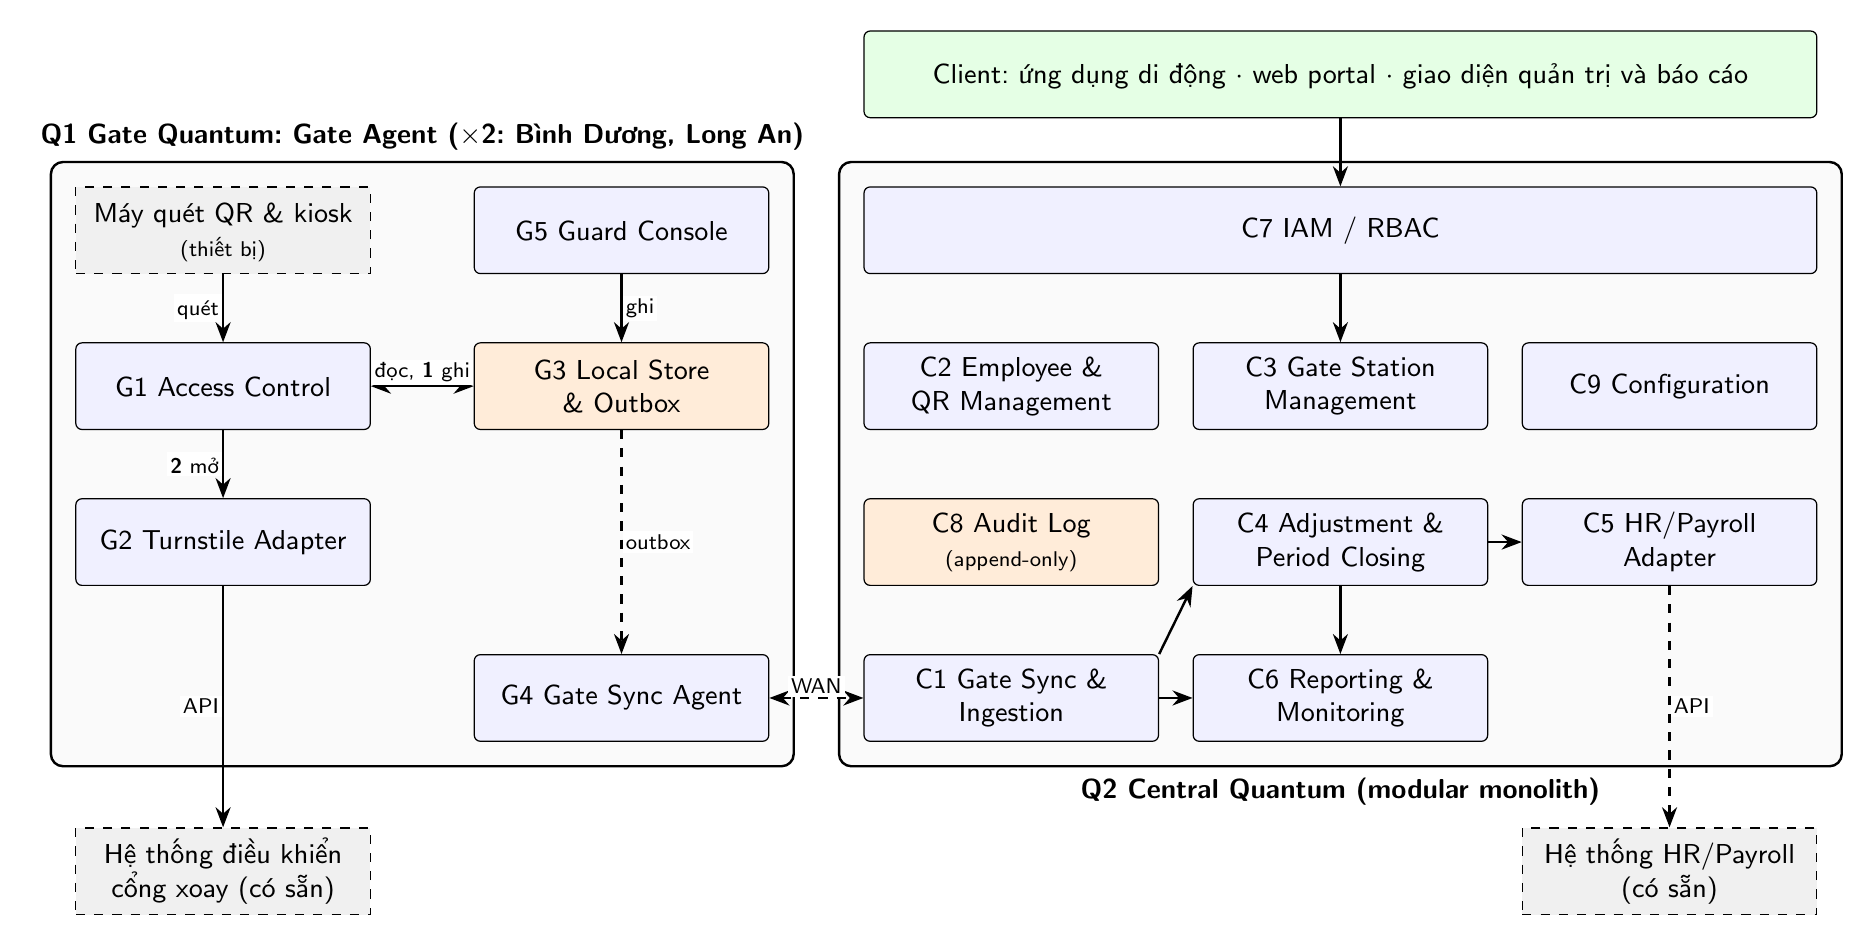
\includegraphics[width=0.9\textwidth]{figures/06_architecture_structure/component_diagram.png}
\caption{Sơ đồ component của hệ thống TMC.}
\label{fig:component_diagram}
\end{figure}

Mũi tên liền là lời gọi đồng bộ; mũi tên đứt là truyền bất đồng bộ.

G5 gọi G2 khi bảo vệ mở cổng thủ công.

Mọi module trung tâm đều ghi vào Audit Log (C8).

C1 lấy danh sách QR hợp lệ từ C2 và lấy cấu hình từ C3, C9 để cấp cho Gate Agent.

\begin{table}[H]
\centering
\small
\renewcommand{\arraystretch}{1.3}
\caption{Cách giao tiếp giữa các component}
\begin{tabularx}{\textwidth}{|>{\raggedright\arraybackslash}p{3.2cm}|>{\raggedright\arraybackslash}p{3.2cm}|>{\raggedright\arraybackslash}X|}
\hline
\textbf{Từ $\rightarrow$ Đến} & \textbf{Kiểu giao tiếp} & \textbf{Interface / nội dung} \\
\hline
Máy quét $\rightarrow$ G1 & Đồng bộ, cục bộ & Sự kiện quét (nội dung QR, mã trạm) \\
\hline
G1 $\rightarrow$ G3 & Đồng bộ, cục bộ & AllowlistReader.find(), TransactionStore.append() \\
\hline
G1, G5 $\rightarrow$ G2 & Đồng bộ, có timeout & TurnstileGateway.open() \\
\hline
G2 $\rightarrow$ Hệ thống cổng xoay & Đồng bộ, mạng nội bộ nhà máy & API cổng xoay (C-01) \\
\hline
G5 $\rightarrow$ G3 & Đồng bộ, cục bộ & Ghi ManualGateOpening \\
\hline
G3 $\rightarrow$ G4 $\rightarrow$ C1 & Bất đồng bộ, giao ít nhất một lần, idempotent theo eventId & Giao dịch, lần quét bị từ chối, mở cổng thủ công, heartbeat \\
\hline
C1 $\rightarrow$ G4 $\rightarrow$ G3 & Bất đồng bộ, kéo định kỳ, trễ $\le$ 60 giây & Danh sách QR hợp lệ, cấu hình trạm \\
\hline
C2, C3, C9 $\rightarrow$ C1 & Domain event trong tiến trình & QrCredentialChanged, StationConfigChanged, SettingChanged \\
\hline
C1 $\rightarrow$ C4, C6 & Domain event trong tiến trình & TransactionRecorded \\
\hline
C4 $\rightarrow$ C6 & Domain event trong tiến trình & AdjustmentRecorded, PeriodStatusChanged \\
\hline
C4 $\rightarrow$ C5 & Bất đồng bộ qua outbox trung tâm & ExportBatchReady \\
\hline
C5 $\rightarrow$ HR/Payroll & Bất đồng bộ theo lô, gửi lại khi lỗi & HrPayrollGateway.submit() (C-01) \\
\hline
Client $\rightarrow$ C7 $\rightarrow$ các module & Đồng bộ, HTTPS & API của từng module; kiểm tra quyền trước khi xử lý \\
\hline
Mọi module $\rightarrow$ C8 & Trong tiến trình, ghi bền vững & AuditLog.record() \\
\hline
\end{tabularx}
\end{table}

F1 – Quét QR qua cổng.

G1 nhận nội dung QR từ máy quét và tra trong danh sách QR hợp lệ ở G3. G1 kiểm tra:

QR ở trạng thái ACTIVE và nhân viên đang hoạt động;

trạm đang bật (INV-03);

lần quét không vi phạm anti-passback (INV-04).

Nếu hợp lệ: G1 ghi AttendanceTransaction kèm eventId vào G3 trước. Chỉ sau đó G1 mới gửi lệnh mở cổng qua G2 và báo thành công trên kiosk (INV-05). Nếu không hợp lệ: G1 ghi ScanAttempt kèm lý do (INV-07) và hiển thị kết quả trên cả kiosk lẫn G5.

Nếu gọi cổng xoay lỗi hoặc quá thời gian: giao dịch đã ghi vẫn giữ nguyên, và bảo vệ xử lý tại G5 bằng cách mở cổng thủ công (FR-09). Nếu nhân viên cuối cùng không qua cổng, HR hủy giao dịch bằng điều chỉnh (FR-15).

Toàn bộ luồng chỉ dùng dữ liệu cục bộ. Phần lớn ngân sách 2 giây dành cho cổng xoay, vốn mất tối đa 500 ms (A-03).

F2 – Đồng bộ giữa hai quantum.

Chiều lên: G4 đọc outbox trong G3 và gửi lên C1. C1 bỏ qua bản trùng theo eventId rồi gửi xác nhận. G4 chỉ đánh dấu một bản ghi là đã gửi khi nhận được xác nhận.

Chiều xuống: G4 kéo danh sách QR hợp lệ và cấu hình trạm về. Khi có mạng, độ trễ không quá 60 giây (INV-02).

Heartbeat: G4 gửi heartbeat định kỳ để C3 phát hiện trạm offline.

F3 – Điều chỉnh và chốt kỳ.

Điều chỉnh: HR điều chỉnh giao dịch qua C4, bắt buộc có lý do. Giao dịch gốc được giữ nguyên (INV-08) và mọi thao tác được ghi vào C8.

Chốt kỳ: đến lịch đặt trong C9, C4 chuyển kỳ sang CLOSED, tạo đợt MAIN và đưa vào outbox trung tâm. C5 gửi đợt này sang HR/Payroll; nếu lỗi thì gửi lại chính đợt đó. Lịch chốt được đặt đủ sớm để còn thời gian dự phòng trước 12:00 ngày 1 (NFR-03). C4 phát cảnh báo nếu đến sát hạn mà đợt MAIN vẫn chưa được HR/Payroll xác nhận.

Sau khi khóa kỳ: khi kỳ đã ở trạng thái LOCKED, mọi điều chỉnh mới đi vào đợt SUPPLEMENTAL (INV-09).

F4 – Gate Agent mất kết nối. Gate Agent vận hành theo Bảng 6.3.3.

\begin{table}[H]
\centering
\small
\renewcommand{\arraystretch}{1.3}
\caption{Hành vi của Gate Agent theo trạng thái kết nối}
\begin{tabularx}{\textwidth}{|>{\raggedright\arraybackslash}p{3.5cm}|>{\raggedright\arraybackslash}X|>{\raggedright\arraybackslash}X|}
\hline
\textbf{Trạng thái} & \textbf{Chiều vào} & \textbf{Chiều ra} \\
\hline
Có kết nối & Bình thường; danh sách QR hợp lệ cập nhật với độ trễ $\le$ 60 giây & Bình thường \\
\hline
Mất kết nối, chưa quá ngưỡng (ngưỡng đặt ở C9) & Vẫn hoạt động bằng dữ liệu cục bộ; dữ liệu tích lại trong outbox; C3 cảnh báo khi mất heartbeat & Bình thường \\
\hline
Mất kết nối, quá ngưỡng & Fail-closed: cổng không tự mở; bảo vệ mở thủ công qua G5 (FR-09, bắt buộc lý do, có audit) & Luôn cho ra vì an toàn cháy nổ; lần quét vẫn được ghi để chấm công \\
\hline
\end{tabularx}
\end{table}

Giá trị ngưỡng mất kết nối sẽ được chốt cùng giảng viên, như đã nêu ở mục 5.2. Khi có mạng trở lại, luồng F2 gửi bù toàn bộ outbox; eventId bảo đảm không tạo bản ghi trùng.

\subsection{Kiến trúc vật lý}
Kiến trúc vật lý xác định cách thức các thành phần Component được ánh xạ và triển khai trên Nodes, môi trường thực thi, cấu hình mạng và đường truyền vật lý, nhằm hiện thực hóa các mục tiêu về hiệu năng, độ tin cậy không mất mát dữ liệu và tính sẵn sàng/ khả năng tự vận hành offline.

\subsubsection{Lựa chọn Topology triển khai}
Hệ thống TMC được quyết định triển khai theo mô hình Hybrid Edge-Central Topology (Kết hợp điện toán biên tại nhà máy và điện toán tập trung tại máy chủ trung tâm):  

Phần xử lý tại từng nhà máy (Edge - Gate Quantum Q1):
\begin{itemize}
    \item Toàn bộ phần mềm quét mã, xác thực và điều khiển mở cổng được cài đặt trực tiếp trên máy tính tại trạm cổng (Kiosk) của 2 nhà máy (Bình Dương và Long An).
    \item Mục đích: Xử lý ngay tại mạng nội bộ để đảm bảo tốc độ phản hồi cực nhanh ($\le$ 2 giây - NFR-01), giải quyết triệt để bài toán ùn tắc giờ cao điểm đổi ca, đồng thời giúp cổng vẫn tự hoạt động bình thường kể cả khi mất kết nối Internet về trung tâm (NFR-07, NFR-10).
\end{itemize}

Phần xử lý tập trung (Central - Central Quantum Q2):
\begin{itemize}
    \item Toàn bộ phần mềm quản lý nhân sự, phân quyền người dùng (RBAC), lưu trữ dữ liệu tổng và đối soát lương được đặt tập trung trên máy chủ trung tâm (Cloud / Datacenter).
    \item Mục đích: Đảm bảo an toàn, nhất quán dữ liệu và kiểm toán tập trung (NFR-02, NFR-04, NFR-05), phục vụ việc tổng hợp báo cáo và truyền dữ liệu sang hệ thống HR/Payroll đúng hạn chốt lương hằng tháng (C-02, NFR-03).
\end{itemize}

\subsubsection{Sơ đồ triển khai vật lý}
Sơ đồ triển khai dưới đây mô tả cấu trúc vật lý, vị trí của từng thành phần, ranh giới mạng và phương thức liên kết giữa các hệ thống:

\begin{figure}[H]
\centering
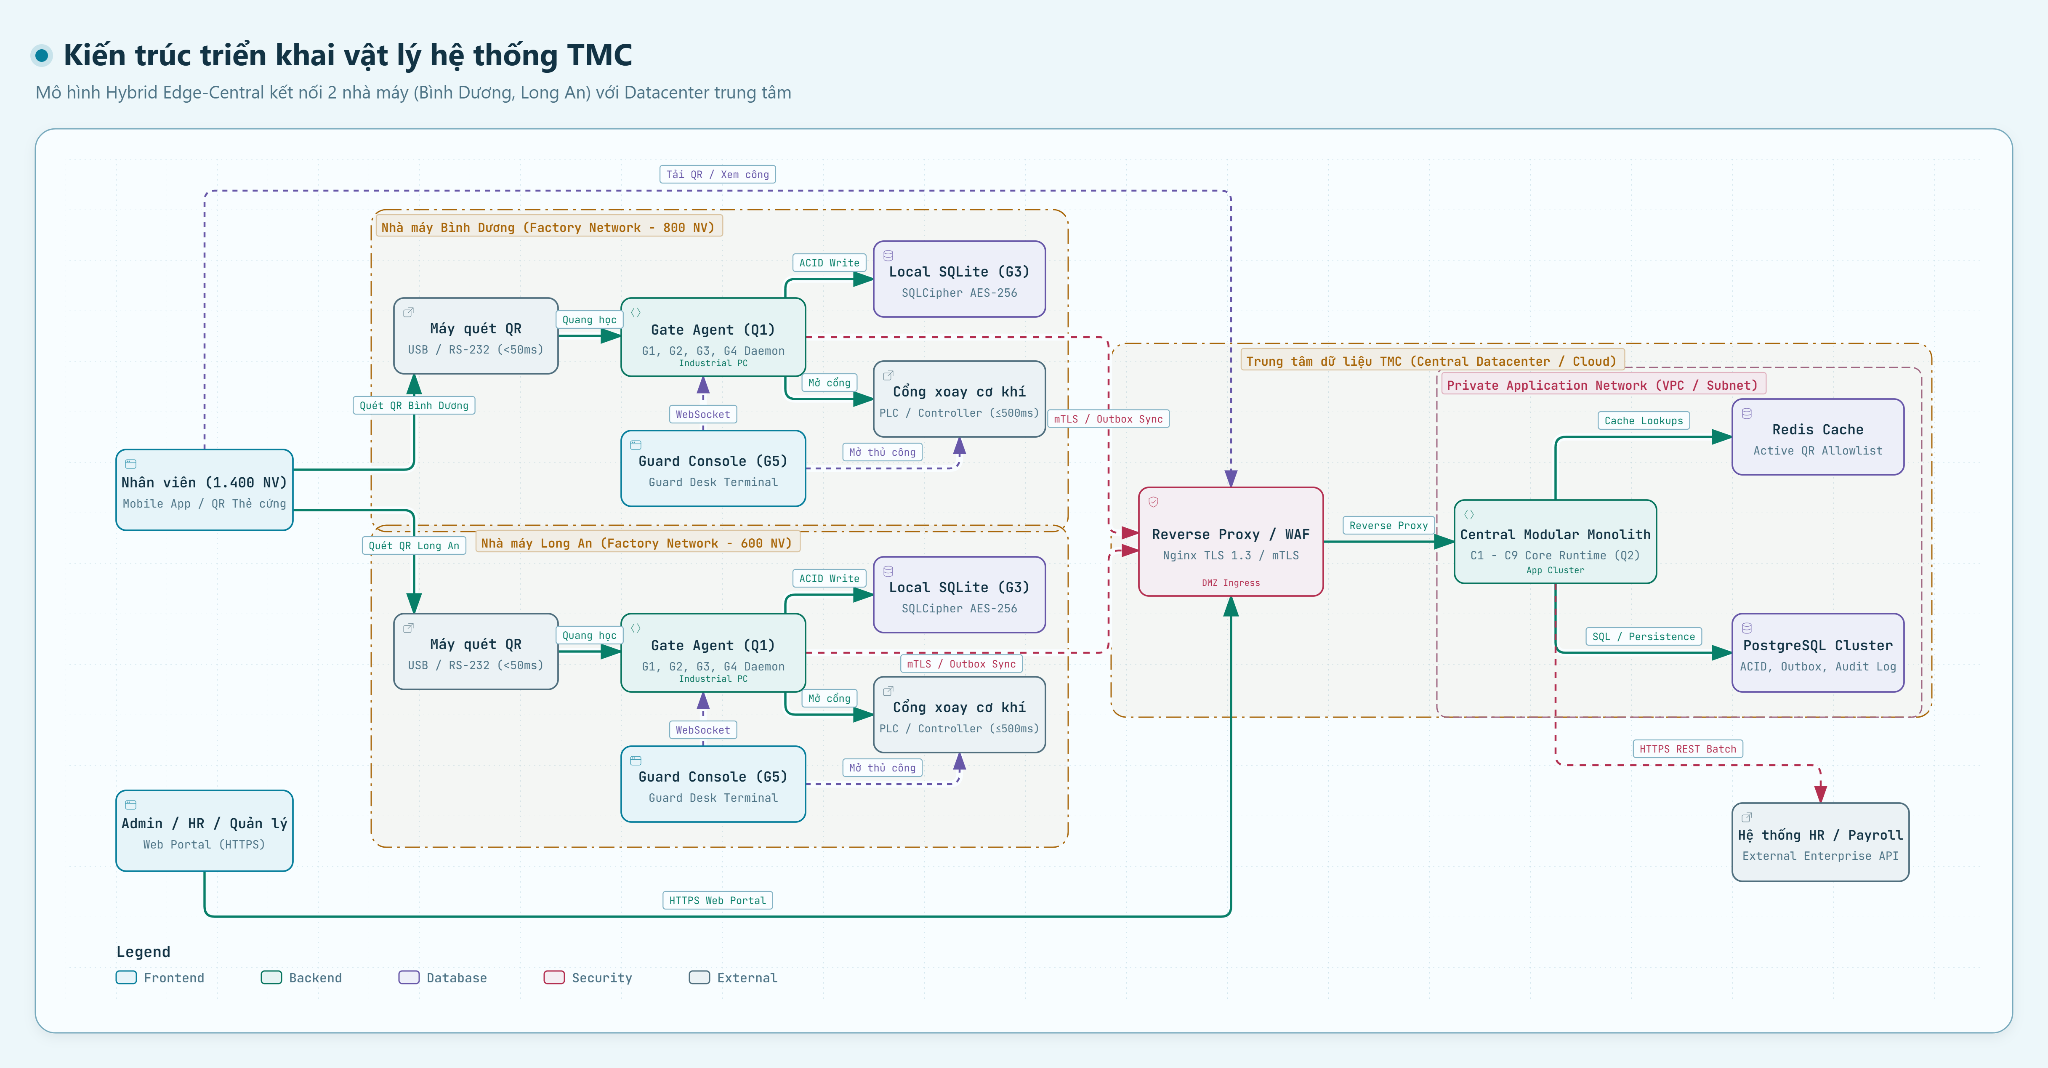
\includegraphics[width=0.95\textwidth]{figures/06_architecture_structure/deployment_diagram.png} 
\caption{Sơ đồ triển khai vật lý hệ thống TMC}
\end{figure}

\subsubsection{Đặc tả chi tiết các Node và Phân bổ Component}
Bảng dưới đây quy định chi tiết cấu hình phần cứng, vai trò môi trường và các component được triển khai trên từng nút mạng:

\small
\renewcommand{\arraystretch}{1.3}
\begin{longtable}{|>{\raggedright\arraybackslash}p{2.8cm}|>{\raggedright\arraybackslash}p{3.0cm}|>{\raggedright\arraybackslash}p{2.6cm}|>{\raggedright\arraybackslash}p{7.2cm}|}
\caption{Đặc tả chi tiết các Node và Phân bổ Component} \\
\hline
\textbf{Tên Node} & \textbf{Môi trường / Phần cứng} & \textbf{Component đảm nhận} & \textbf{Vai trò và Đặc tính kỹ thuật} \\
\hline
\endfirsthead

\hline
\textbf{Tên Node} & \textbf{Môi trường / Phần cứng} & \textbf{Component đảm nhận} & \textbf{Vai trò và Đặc tính kỹ thuật} \\
\hline
\endhead

\hline
\multicolumn{4}{r}{\textit{Còn tiếp sang trang sau...}} \\
\hline
\endfoot

\hline
\endlastfoot

Gate Station Kiosk Node (Tại mỗi cổng/nhà máy) & Industrial Mini PC (Linux Ubuntu Core / Alpine), RAM 4GB, 64GB SSD, Dual NIC (Ethernet). Gắn máy quét QR quang học và màn hình phụ. & G1 (Access Control), G2 (Turnstile Adapter), G3 (Local Store \& Outbox), G4 (Gate Sync Agent) & Chạy như một Service/Daemon độc lập trên Linux. Đảm bảo tính tự chủ tuyệt đối (DP-01). CSDL cục bộ dùng SQLite được mã hóa bằng SQLCipher (AES-256) để bảo vệ dữ liệu cục bộ (NFR-06). Giao tiếp quét mã qua cổng Serial RS-232 / USB HID với độ trễ $<$ 50ms. \\
\hline
Guard Desk Terminal (Tại phòng bảo vệ) & Máy tính bảng công nghiệp / PC màn hình cảm ứng, kết nối mạng LAN nội bộ nhà máy. & G5 (Guard Console - Web Frontend) & Ứng dụng Web tĩnh gọn nhẹ (Single Page Application) phục vụ giám sát luồng quẹt thẻ thời gian thực, hiển thị các bản ghi bị từ chối và thực hiện chức năng mở cổng thủ công khi xảy ra sự cố ngoại lệ (FR-09). \\
\hline
Turnstile Controller Node (Hệ thống ngoài) & Bộ điều khiển phần cứng của cổng xoay (PLC/Controller) do nhà cung cấp thiết bị lắp đặt. & Hệ thống Cổng xoay bên ngoài & Nhận tín hiệu điều khiển mở chốt cơ khí từ G2 qua giao thức TCP/IP Socket hoặc HTTP REST nội bộ LAN. Thời gian phản hồi phần cứng cam kết $\le$ 500ms (A-03). \\
\hline
DMZ Edge Gateway / Reverse Proxy (Trung tâm) & VM Linux cấu hình tối thiểu 2 vCPU, 4GB RAM, triển khai Nginx / HAProxy. & Reverse Proxy, SSL Termination, WAF & Đóng vai trò cổng vào duy nhất (Single Point of Ingress) cho Central Datacenter. Chấm dứt TLS 1.3, kiểm tra xác thực hai chiều mTLS đối với các Gate Agent (G4), định tuyến API và ngăn chặn tấn công DoS/DDoS. \\
\hline
Central Application Server Node (Trung tâm) & Cluster Container (Docker/K8s) hoặc VM Linux 4 vCPU, 8GB-16GB RAM. & C1 đến C9 (Central Modular Monolith) & Thực thi toàn bộ logic điều phối trung tâm. Triển khai theo mô hình Modular Monolith, các module giao tiếp In-process qua Application Events. Tách biệt thread pool giữa Ingestion (C1), Xử lý nghiệp vụ (C2, C3, C4) và Báo cáo (C6). \\
\hline
Central Database Server Node (Trung tâm) & Hệ quản trị CSDL Quan hệ PostgreSQL (Primary - Standby Replica). & Lưu trữ tập trung toàn bộ dữ liệu nghiệp vụ, Audit Log (C8), Read Model (C6) & Đảm bảo tính nhất quán mạnh (ACID) cho việc chốt kỳ, quản lý nhân viên, và lưu trữ lịch sử chấm công tập trung. Bảng audit\_log được cấu hình Append-Only và phân vùng theo thời gian (Partitioning by Month). \\
\hline
Central Cache Server Node (Trung tâm) & Redis Standalone / Cluster in-memory. & Cache danh mục QR hợp lệ, Session tài khoản RBAC & Tăng tốc độ đọc cho các tác vụ tra cứu QR của nhân viên và xác thực token JWT người dùng quản trị. \\
\end{longtable}
\normalsize

\subsubsection{Phân vùng mạng và Giao thức giao tiếp}
1. Mạng Cục bộ Nhà máy (Factory OT/LAN Network - Subnet riêng):
\begin{itemize}
    \item Kết nối giữa Kiosk và Turnstile Controller: Sử dụng mạng LAN cô lập vật lý hoặc VLAN chuyên dụng (VLAN IoT/OT). Giao thức điều khiển là HTTP/REST hoặc TCP Socket với địa chỉ IP tĩnh. Không cho phép truy cập Internet trực tiếp từ dải mạng này.
    \item Giao tiếp giữa G5 (Guard Console) và Kiosk: HTTP/WebSocket cục bộ qua LAN.
\end{itemize}

2. Mạng Diện rộng Kết nối Nhà máy - Trung tâm (WAN / VPN Tunnel):
\begin{itemize}
    \item Kênh truyền từ G4 (Gate Sync Agent) tại các nhà máy lên C1 (Gate Sync \& Ingestion) tại Trung tâm được bảo vệ thông qua đường truyền Site-to-Site IPSec VPN hoặc kênh mã hóa HTTPS/TLS 1.3 trên nền Internet công cộng.
    \item Cơ chế xác thực thiết bị: Sử dụng mTLS (Mutual TLS) với chứng chỉ số X.509 riêng biệt được nạp an toàn vào từng Kiosk phần cứng, ngăn chặn triệt để hành vi giả mạo Gate Agent để inject dữ liệu chấm công.
\end{itemize}

3. Mạng Tích hợp Hệ thống HR/Payroll:
\begin{itemize}
    \item C5 gọi sang API của Hệ thống HR/Payroll qua kênh truyền mạng riêng (Dedicated Leased Line / MPLS) hoặc HTTPS REST API bảo vệ bằng IP Whitelisting và OAuth 2.0 / Mutual TLS.
\end{itemize}